\chapter{Generating signed snarks}

Since the structure of snarks is generally unknown, brute force is still the best approach. Considering one underlying graph, the number of signed graphs is simply too big for an efficient analysis. Filtering them up to switching-isomorphism reduces these numbers to manageable amounts and ensures clean and usable data. Bagheri, Moghaddamfar, Ramezani \cite{switching-isomorphic} establish a method of determining the non-switching-isomorphic signed graphs based on the action of its automorphism group. Our aim is to automate this process using a different idea and making analysis of small cubic signed graphs possible.

\section{Switching equivalence}

Recall that two signed graphs $\Gamma \sim \Sigma$ are \textit{switching-equivalent} if a switching function $\theta$ exists such that $\Gamma ^{\theta} = \Sigma$. Given an underlying graph $G$ there are $2^{|E_G|}$ possible signed graphs constructed from $G$. However, provided that $G$ is connected, only $2^{|E_G| - |V_G| + 1}$ of them are mutually non-switching-equivalent.

\begin{theorem}\label{lem1:eq-classes}
    Let $G$ be a simple unsigned connected graph with $n$ vertices and $m$ edges. There are $2^{m - n + 1}$ mutually non-switching-equivalent graphs based on $G$.
\end{theorem}

\textit{Proof.} Bagheri, Moghaddamfar, Ramezani\cite{switching-isomorphic} prove this theorem in a different way but we present a version that is actually used in the implementation. The idea is to use a spanning tree $S$ of graph $G$ and show that each switching equivalence class of $G$ has exactly one element that is all-positive on $S$. Since $S$ contains $n - 1$ edges, there are $2^{m - (n - 1)}$ different signed graphs all-positive on $S$. Suppose we have a signed graph $\Gamma$ all-positive on $S$ and we switch some vertices. If we switch no vertices or all vertices, the graph stays the same, so we will have a non-empty set of switched vertices $A$ and a non-empty set of unswitched vertices $B$. At least one edge of $S$ must have one end in $A$ and the other end in $B$, otherwise $G$ would not be connected or $S$ would not be a spanning tree. After this switching all edges with both ends in either $A$ or $B$ will retain the same sign (not reversed or reversed twice) and edges with one end in $A$ and on end in $B$ will have its sign reversed. Therefore every possible switching from $\Gamma$ that would change the signature will result in a graph that is not all-positive on $S$. \qed

We use this approach to reduce the number of signed graphs that need to be filtered for isomorphisms.

\section{Switching isomorphism}

Two signed graphs $\Gamma _1$ and $\Gamma _2$ are \textit{isomorphic} if a bijection $\phi : V _{\Gamma _1} \rightarrow V _{\Gamma _2}$ exists that preserves vertex adjacency and edge signs.

$$(\forall u,v \in V _{\Gamma}) ~~ uv \in E _{\Gamma _1} \iff \phi(u)\phi(v) \in E _{\Gamma _2}$$
$$(\forall e = uv \in E _{\Gamma}) ~~ \sigma _{\Gamma _1} (uv) = \sigma _{\Gamma _2} (\phi(u)\phi(v))$$

Two graphs are \textit{switching isomorphic} if one graph is isomorphic to a switching equivalent of the other. This is the natural definition but in the generating algorithm and its proof of correctness we will be referring to an equivalent definition using the balance of cycles.

\begin{lemma}\label{lem:cycle-switching}
    Two connected signed graphs $\Gamma _1 = (G, \sigma _1)$ and $\Gamma _2 = (G, \sigma _2)$ with the same underlying graph are switching equivalent if and only if all cycles in $G$ have the same balance in $\Gamma _1$ and $\Gamma _2$.
\end{lemma}

\textit{Proof.} We already know that switching doesn't change the balance of cycles so switching equivalence trivially implies cycle balance consistency. Now suppose we have two graphs with the same underlying graph and the same balance of each cycle. Let $S$ again be a spanning tree of $G$. Based on \cref{lem1:eq-classes} each equivalence class has exactly one signature that is all-positive on $S$ so we will switch both graphs to their respective signatures that are all-positive on $S$. Each cycle has exactly one edge outside of $S$ and since $S$ is all-positive the balance of each cycle is determined by the sign of this one edge. In other words, there is a one-to-one correspondence between the balance of cycles and signature of edges outside of $S$. Each cycle has the same balance in both graphs, therefore each edge outside of $S$ has the same sign in both graphs. Each edge in $S$ also has the same signature in both graphs of course so the signatures are identical and $\Gamma _1$ and $\Gamma _2$ are switching equivalent. \qed

\begin{theorem}\label{th:cycle-isomorphic}
    Let $\mathcal{C} (\Gamma)$ denote the set of all cycles in $\Gamma$. Two signed graphs $\Gamma _1 = (G_1, \sigma _1)$ and $\Gamma _2 = (G_2, \sigma _2)$ are switching isomorphic if a bijection $\phi : V _{\Gamma _1} \rightarrow V _{\Gamma _2}$ exists such that

    $$(\forall u,v \in V _{\Gamma _1}) ~~ uv \in E _{\Gamma _1} \iff \phi(u)\phi(v) \in E _{\Gamma _2}$$

    $$(\forall c = v_0v_1v_2 \dots v_k \in \mathcal{C} (\Gamma _1); v_0 = v_k)$$
    $$\sigma _1 (v_0v_1)\sigma _1 (v_1v_2) \dots \sigma _1 (v_{k-1}v_k) = \sigma _2 (\phi(v_0)\phi(v_1))\sigma _2 (\phi(v_1)\phi(v_2)) \dots \sigma _2 (\phi(v_{k-1})\phi(v_k))$$

    In other words, instead of preserving edge signs the bijection preserves cycle balance.
\end{theorem}

\textit{Proof}. Follows mostly from \cref{lem:cycle-switching} with one exception. The definition by itself doesn't preserve the signs of edges that are not part of any cycle, i.e. \textit{bridges} (edges whose removal disconnects the graph). However, we can always reverse the sign of a bridge "for free" by switching all vertices on one side of the bridge. The only edge that changes signs is the actual bridge. Thus in the context of switching isomorphism the sign of bridges is irrelevant. \qed

The \textit{cycle space} $\mathcal{E} (\Gamma)$of a graph is the collection of its even-degree spanning subgraphs. It can be described as a vector space over the two-element Galois field: the elements are even-degree subgraphs as vectors over $\mathbb{Z} _2$. The additive operation is the symmetric difference from the subgraph perspective (given two even-degree subgraphs $A$ and $B$, $A \oplus B$ contains edges that are in either $A$ or $B$ but not both) and simple sum from $\mathbb{Z} _2$ perspective. Scalar multiplication is trivially defined, multiplication by 0 yields a graph with no edges (zero in the cycle space) and multiplication by 1 is identity. Cycles are trivial elements of the cycle space because each even-degree subgraph is the sum of some cycles in the context of this vector space. Consequently, there must be a \textit{cycle basis}, a set of linearly independent cycles that generates the entire cycle space.

\subsection{Transformation}

\begin{figure}[h]\label{fig:transformation}
    \centering
    \begin{tikzpicture}
        \begin{scope}[every node/.style={circle,draw}]
            \node (1)  at (0,0) {1};
            \node (2)  at (3,0) {2};
            \node (3)  at (0,-3) {3};
            \node (4)  at (3,-3) {4};
        \end{scope}
        \node (cheat) at (-1.5,1.2) {};
        \node (cheat2) at (3.8,-5.2) {};
        \node (desc) at (1.5,1) {$\Gamma$};
        \begin{scope}[every edge/.style={draw,very thick}]
            \path
                (1) edge (2)
                (2) edge [dashed] (3)
                (3) edge (1)
                (2) edge (4)
                (3) edge [dashed] (4);
        \end{scope}
    \end{tikzpicture}
    \hspace{0.1\textwidth}
    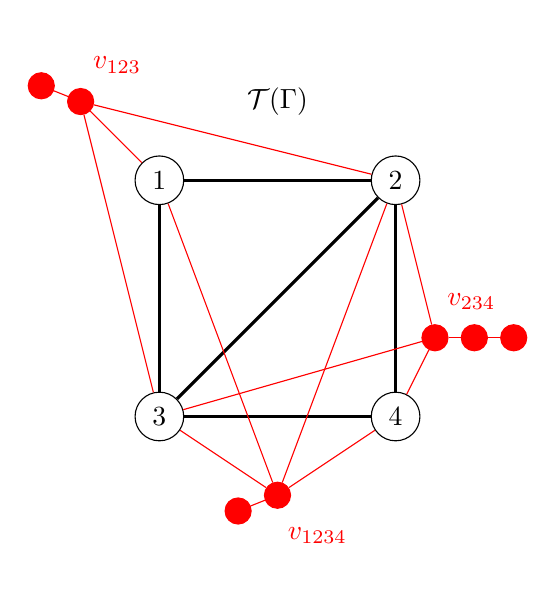
\begin{tikzpicture}
        \begin{scope}[every node/.style={circle,draw}]
            \node (1)  at (0,0) {1};
            \node (2)  at (3,0) {2};
            \node (3)  at (0,-3) {3};
            \node (4)  at (3,-3) {4};
        \end{scope}
        \begin{scope}[every node/.style={circle,draw,color=red,fill=red}]
            \node (11) [label={above right:$v_{123}$}]  at (-1,1) {};
            \node (12) [label={above right:$v_{234}$}] at (3.5,-2) {};
            \node (13) [label={below right:$v_{1234}$}] at (1.5,-4) {};
            \node (14) [] at (4,-2) {};
            \node (15) [] at (4.5,-2) {};
            \node (16) [] at (-1.5,1.2) {};
            \node (17) [] at (1,-4.2) {};
        \end{scope}
        \node (desc) at (1.5,1) {$\mathcal{T} (\Gamma)$};
        \begin{scope}[every edge/.style={draw,very thick}]
            \path
                (1) edge (2)
                (2) edge (3)
                (3) edge (1)
                (2) edge (4)
                (3) edge (4);
        \end{scope}
        \begin{scope}[every edge/.style={draw,thin,color=red}]
            \path
                (1) edge (11)
                (2) edge (11)
                (3) edge (11)
                (11) edge (16);
        \end{scope}
        \begin{scope}[every edge/.style={draw,thin,color=red}]
            \path
                (2) edge (12)
                (3) edge (12)
                (4) edge (12)
                (12) edge (14)
                (14) edge (15);
        \end{scope}
        \begin{scope}[every edge/.style={draw,thin,color=red}]
            \path
                (1) edge (13)
                (2) edge (13)
                (3) edge (13)
                (4) edge (13)
                (13) edge (17);
        \end{scope}
    \end{tikzpicture}
    \caption[Transformation to an unsigned graph preserving cycle balance]{Transformation to an unsigned graph preserving cycle balance.}
\end{figure}

The following transformation of signed graphs to unsigned graphs preserves switching isomorphism and allows us to use existing tools to determine whether two signed graphs are switching isomorphic.

\begin{theorem}\label{th:conversion}
    From a connected signed graph $\Gamma$ we will construct an unsigned graph $\mathcal{T} (\Gamma)$ in the following way. Starting with the underlying graph, for each cycle $c$ in $\mathcal{C} (\Gamma)$ we add one \textit{cycle vertex} $v_c$ and connect it to each vertex of the original cycle. We represent their balance with \textit{"tails"}, i.e. one or two new vertices connected to the cycle vertex, $a_c$ and possibly $b_c$. Cycle vertices for balanced cycles will have a tail of length one and for unbalanced cycles a tail of length two.

    Signed graphs $\Gamma _1$ and $\Gamma _2$ with minimal degree three or more are switching isomorphic if and only if $\mathcal{T} (\Gamma _1)$ and $\mathcal{T} (\Gamma _2)$ are isomorphic.
\end{theorem}

\textit{Proof.} The tails are either a vertex of degree one or an additional vertex of degree two. Since degrees of vertices are preserved under isomorphism and both original vertices and cycle vertices have degree at least three, balanced tails will be projected only onto balanced tails and unbalanced tails onto unbalanced tails. By extension cycle vertices will be projected only onto other cycle vertices, because each tail is connected to exactly one cycle vertex. Consequently the original vertices will also be projected only onto each other.

Suppose there is a switching isomorphism $\phi$ between $\Gamma _1$ and $\Gamma _2$. We will construct an isomorphism $\psi$ between $\mathcal{T} (\Gamma _1)$ and $\mathcal{T} (\Gamma _2)$. For each $v \in V_{\Gamma _1}$ there is a vertex $v$ in $\mathcal{T} (\Gamma _1)$ and we put $\psi (v) = \phi (v)$. For each cycle $c = v_0v_1v_2 \dots v_k \in \mathcal{C} (\Gamma _1); ~ v_0 = v_k; ~ v_i \in V_{\Gamma _1}$ there will again be a cycle $c ^{\phi} = \phi(v_0)\phi(v_1)\phi(v_2) \dots \phi(v_k) \in \mathcal{C} (\Gamma _2); ~ \phi(v_0) = \phi(v_k); ~ \phi(v_i) \in V_{\Gamma _2}$ in $\Gamma _2$ with the same balance by definition of switching isomorphism. Consequently, there will again be cycle vertices $v_c \in \mathcal{T} (\Gamma _1)$ and $v_{c ^{\phi}} \in \mathcal{T} (\Gamma _2)$ with tails of the same length because of the same balance of $c$ and $c ^{\phi}$, so we can put $\psi (v_c) = v_{c ^{\phi}}$, $\psi (a_c) = a_{c ^{\phi}}$ and possibly $\psi (b_c) = b_{c ^{\phi}}$ (recall that $a_c$ and $b_c$ are tail vertices of $v_c$). Based on the definition of $\mathcal{T}$ here are no other vertices in $\mathcal{T} (\Gamma _1)$ or $\mathcal{T} (\Gamma _2)$ and so $\psi$ is an isomorphism between $\mathcal{T} (\Gamma _1)$ and $\mathcal{T} (\Gamma _2)$.

Now suppose that $\mathcal{T} (\Gamma _1)$ and $\mathcal{T} (\Gamma _2)$ are isomorphic and let $\psi$ be their bijection. As shown above, $\psi$ reduced to $V_{\Gamma _1}$, let's call it $\phi ^*$, will be an isomorphism between $\Gamma _1$ and $\Gamma _2$ that doesn't preserve edge signs. So for each cycle $c = v_0v_1v_2 \dots v_k \in \mathcal{C} (\Gamma _1); ~ v_0 = v_k; ~ v_i \in V_{\Gamma _1}$ there will be a cycle $c ^{\phi ^*} = \phi ^*(v_0)\phi ^*(v_1)\phi ^*(v_2) \dots \phi ^*(v_k) \in \mathcal{C} (\Gamma _2); ~ \phi ^*(v_0) = \phi ^*(v_k); ~ \phi ^*(v_i) \in V_{\Gamma _2}$ (recall that original vertices can be projected only onto original vertices). Based on the definition of $\mathcal{T}$, $\mathcal{T} (\Gamma _1)$ will have a cycle vertex $v_c$ connected to each vertex in $c$ and $\mathcal{T} (\Gamma _2)$ will have a cycle vertex $v_{c^{\phi ^*}}$ connected to each vertex in $c^{\phi ^*}$. It must be true that $\psi (v_c) = v_{c^{\phi ^*}}$, otherwise there is another vertex $\psi (v_c)$ in $\mathcal{T} (\Gamma _2)$ that is connected to all vertices of $c ^{\phi ^*}$, which would mean that there are two cycles with the same vertices in $\Gamma _2$, which is a contradiction. The projection of the tail of $v_c$ must be the tail of $v_{c^{\phi ^*}}$ for the same reason, by definition of $\mathcal{T} ()$ a cycle vertex only has one tail. Finally, due to the nature of the transformation $c$ and $c ^{\phi ^*}$ must have the same balance. \qed

\begin{lemma}\label{lem:genset}
    Let $\mathcal{C} ^* (\Gamma)$ be the set of all cycles in $\Gamma$ with length up to some $n$ such that this set generates the cycle space $\mathcal{E} (\Gamma)$. When using this set of cycles instead of all cycles in $\mathcal{T} (\Gamma)$, \cref{th:conversion} still holds.
\end{lemma}

We are using a generating subset of $\mathcal{E} (\Gamma)$ (which is also the generating subset of $\mathcal{C} (\Gamma)$) to be more efficient. If a cycle $c$ is the sum of some cycles in $\mathcal{C} ^* (\Gamma)$, their balance directly determines the balance of $c$. So any isomorphism that preserves the balance of $\mathcal{C} ^* (\Gamma)$ will preserve the balance of $\mathcal{C} (\Gamma)$ as well.

It is, however, necessary to use all cycles of length up to $n$ for $\mathcal{T}$ because of the nature of isomorphism. In theory we would only need an isomorphism that preserves the balance of any cycle basis in $\Gamma _1$ because if $\Gamma _1$ and $\Gamma _2$ are isomorphic, $\mathcal{E} (\Gamma _1)$ and $\mathcal{E} (\Gamma _2)$ are also isomorphic and the projection of any basis in $\mathcal{E} (\Gamma _1)$ will be a basis in $\mathcal{E} (\Gamma _2)$. The issue with this approach is that it doesn't guarantee that cycles of the same length will be projected onto each other, which is required by $\mathcal{T}$.

\section{Coloring}

To determine the chromatic index of a cubic graph is an NP-complete problem. By extension, determining the chromatic index of a signed cubic graph is also NP-complete, because of the trivial reduction from the signed chromatic index problem to the unsigned chromatic index problem. Instead of designing an algorithm we decided to implement a conversion from the chromatic index problem to 3SAT and using a highly optimized SAT solver in the hope for better effectiveness.

\subsection{Conversion to 3SAT}

For any cubic signed graph $\Gamma$ we will construct a 3SAT formula $F(\Gamma)$ that is satisfiable if and only if the graph is 3-colorable. There will be three literals for each half-edge $ev \in \Sigma _{\Gamma}$, one for each colour from $C_3 = \{-1, 0, 1\}$. Let's call them $x^{-1}_{ev}$, $x^{0}_{ev}$ and $x^{1}_{ev}$. In any evaluation of these literals that satisfy $F$ exactly one of them will be true denoting the colour of the half-edge. This will be guaranteed using three constituent formulas. Let $\Gamma = (G, \sigma)$

$$F_1 (\Gamma) = \bigwedge _{e = vw \in E_{\Gamma}} (x^{-1}_{ev} \vee x^{0}_{ev} \vee x^{1}_{ev}) \wedge (x^{-1}_{ew} \vee x^{0}_{ew} \vee x^{1}_{ew}) $$

The first formula ensures that each half-edge is coloured and is the only one containing clauses of length 3. The next formula will enforce the correctness of the colouring, restricting the colours of half edges that form one complete edge. Illegal signatures for each edge are negated using DeMorgan rules, resulting in a convenient CNF form. No edge can be coloured $0$ on one side and $1$ or $-1$ on the other

$$F_{abs} (e = vw) = \neg (x^{0}_{ev} \land x^{1}_{ew}) \land \neg (x^{1}_{ev} \land x^{0}_{ew}) \land \neg (x^{0}_{ev} \land x^{-1}_{ew}) \land \neg (x^{-1}_{ev} \land x^{0}_{ew})$$
$$F_{abs} (e = vw) = (\neg x^{0}_{ev} \lor \neg x^{1}_{ew}) \land (\neg x^{1}_{ev} \lor \neg x^{0}_{ew}) \land (\neg x^{0}_{ev} \lor \neg x^{-1}_{ew}) \land (\neg x^{-1}_{ev} \lor \neg x^{0}_{ew})$$

and the colours must be the same if the edge is positive and opposite if the edge is negative, which is equivalen to the following.

$$F _{sign} (e = vw) = (\neg x^{-1}_{ev} \lor \neg x^{\sigma (e, w)}_{ew}) \land (\neg x^{1}_{ev} \lor \neg x^{-\sigma (e, w)}_{ew})$$

$$F_2 (\Gamma)= \bigwedge _{e = vw \in E_{\Gamma}} F _{abs} (e) \wedge F _{sign} (e)$$

Lastly we need to ensure that the colouring is proper. Let $N(v) = \{e ~|~ (e,v) \in \Sigma _{\Gamma}\}$ be the set of half-edges incident to $v$.

$$F_3 (\Gamma)= \bigwedge _{\substack{v \in V_{\Gamma} \\ e_1, e_2 \in N(v); ~ e_1 \neq e_2}} (\neg x^{-1}_{e_1v} \lor \neg x^{-1}_{e_2v}) \land (\neg x^{0}_{e_1v} \lor \neg x^{0}_{e_2v}) \land (\neg x^{1}_{e_1v} \lor \neg x^{1}_{e_2v}) $$

Each pair of half-edges with a common vertex must have different colours.

\begin{theorem}
    3SAT formula $F(\Gamma) = F_1 (\Gamma) \wedge F_2 (\Gamma) \wedge F_3 (\Gamma)$ constructed in the way described above is satisfiable if and only if $\Gamma$ is 3-colourable.
\end{theorem}

\textit{Proof.} Follows from the construction of $F$ encapsulating all properties of a proper signed 3-colouring. \qed

Note that we don't need to explicitly ensure that for each half-edge exactly one literal is true, in case where multiple literals for different colors are true for the same edge we could choose any color from among them and the coloring would be proper.

\section{Implementation}

The programming language of choice was C++ due to its speed and convenience. Nauty \cite{nauty} is a program for computing the automorphism group of graphs and most importantly the \textit{canonical labeling}. Kissat \cite{kissat}, the winner of the SAT competition 2024, is a simple and fast SAT solver with easy integration.

\subsection{Data structures}

\todo{}
